\documentclass[11pt,a4paper]{article}
\usepackage[a4paper,left=22mm,right=22mm,top=20mm,bottom=21mm]{geometry}
\usepackage{fontspec}
\setmainfont{Times New Roman}
\setsansfont{Arial}
\setmonofont[Scale=0.87]{Consolas}
\usepackage[russian]{babel}
\usepackage{amsmath,amssymb,mathtools}
\usepackage{graphicx,booktabs,tabularx,array}
\usepackage{float}
\usepackage{enumitem}
\usepackage{microtype}
\usepackage{xcolor}
\usepackage{caption}
\usepackage{needspace}
\usepackage[unicode,colorlinks=true,linkcolor=blue!45!black,urlcolor=blue!45!black]{hyperref}
\graphicspath{{../figures/}}
\setlength{\parindent}{1.2em}
\setlength{\parskip}{3pt}
\setlength{\emergencystretch}{2em}
\setlist{nosep,leftmargin=1.7em,topsep=4pt}
\captionsetup{font=small,labelfont=bf}
\newcommand{\code}[1]{\texttt{\detokenize{#1}}}
\newcommand{\R}{\mathbb{R}}
\newcommand{\E}{\mathcal{E}}
\newcommand{\N}{\mathcal{N}}
\DeclareMathOperator{\MSE}{MSE}
\DeclareMathOperator{\Std}{Std}
\DeclareMathOperator{\sign}{sign}
\DeclareMathOperator{\clip}{clip}
\newcommand{\titleblock}[2]{\begin{center}{\Large\bfseries #1\par}\vspace{5pt}{\normalsize #2\par}\end{center}\vspace{4pt}}

\begin{document}
\titleblock{Восстановление графа по матрице наблюдений}{Описание реализованного алгоритма · MNIST · версия для разбора кода}

Задача состоит в выборе соседей каждого признака по множеству наблюдений.
В MNIST наблюдение --- изображение, признак --- яркость пикселя.
Один и тот же неизвестный порядок пикселей используется во всех изображениях.
Алгоритм строит общий неориентированный граф: ребро разрешает использовать
одну вершину для линейного предсказания другой.
Результат представляет разреженный граф предсказательных зависимостей между признаками.

\section{Последовательность действий}
\begin{enumerate}
\item Разделить изображения на обучающую и проверочную части для восстановления структуры.
\item По обучающей части выделить активные признаки и стандартизовать их значения.
\item Вычислить корреляции всех активных пар; для каждой вершины оставить $K$ кандидатов.
\item Построить локальные Lasso-модели, выбрать их регуляризацию по BIC и получить варианты стартового графа.
\item Оценить варианты через Ridge-предсказание на проверочной части и штраф за рёбра.
\item Удалить рёбра, удаление которых уменьшает энергию.
\item Изменять граф стохастическими добавлениями и удалениями, сохраняя лучшее найденное состояние.
\item Вернуться к лучшему состоянию, повторить удаление вредных рёбер и вернуть граф.
\end{enumerate}
\begin{center}
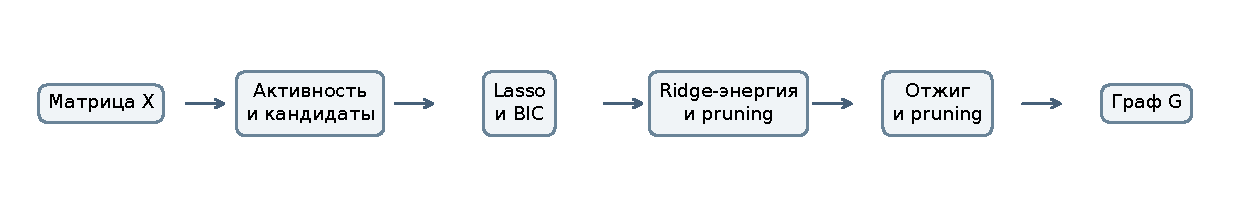
\includegraphics[width=.96\linewidth]{pipeline.pdf}
\end{center}

\section{Данные и обозначения}
Вход: $X^{\rm tr}\in\R^{n\times N}$ и $X^{\rm val}\in\R^{m\times N}$.
Строки --- наблюдения, столбцы --- одни и те же вершины.
Граф $G=(V,E)$ содержит $N$ вершин; $V_a\subseteq V$ --- активное множество,
$p=|V_a|$, $\N_G(i)$ --- соседи вершины $i$. Рёбра неориентированные, без петель.
Неактивные вершины возвращаются изолированными.
\par Алгоритм получает только эти две матрицы и параметры.
Координаты, метки цифр, эталонные рёбра и их количество не передаются.
Входное API: \code{recover_graph(X_train, X_val, config)} в \code{src/latent_graph.py}.

\section{Активные вершины и нормировка}
На обучающей части вычисляются среднее $\mu_i$, стандартное отклонение $\sigma_i$
и частота заметных значений $f_i$:
\begin{equation}
 f_i=\frac1n\sum_{s=1}^n\mathbf1\{|X^{\rm tr}_{si}|>\tau_x\},\qquad
 V_a=\{i:\sigma_i>\tau_\sigma,\ f_i>\tau_f\}.
\end{equation}
Имя \code{variance_threshold} в коде историческое: порог сравнивается
со \emph{стандартным отклонением}, а не с дисперсией.
Для MNIST после деления яркости на 255 используются
$\tau_\sigma=0.02$, $\tau_x=0.05$, $\tau_f=0.01$.
Для $i\in V_a$ обе части нормируются одними обучающими статистиками:
\begin{equation}
 Z^{\rm tr}_{si}=\frac{X^{\rm tr}_{si}-\mu_i}{\sigma_i},\qquad
 Z^{\rm val}_{si}=\frac{X^{\rm val}_{si}-\mu_i}{\sigma_i}.
\end{equation}
Почти постоянный признак не даёт достаточной вариативности для надёжного выбора соседей.
Фильтрация оставляет вершины с достаточной вариативностью наблюдений.

\section{Все пары и список кандидатов}
На всей обучающей части вычисляется корреляция $\rho_{ij}$.
Её строки также случайно делятся на $B=4$ блока, и в каждом вычисляется $\rho^{(b)}_{ij}$.
Все блоки содержат те же столбцы. Оценка пары равна
\begin{equation}
 s_{ij}=\frac{|\rho_{ij}|\,
 \left|B^{-1}\sum_{b=1}^B\sign(\rho^{(b)}_{ij})\right|}
 {1+\Std_b\bigl(|\rho^{(b)}_{ij}|\bigr)}.
\end{equation}
Согласованность знаков повышает оценку, изменчивость модуля её понижает.
В текущем исходнике неопределённая корреляция постоянного столбца внутри блока
заменяется нулём. Эта защитная обработка была добавлена после исторических MNIST-прогонов.
\par Для каждой вершины $i$ множество $C_i$ содержит $K=24$ других вершины с наибольшими $s_{ij}$.
Объединение неориентированных пар $(i,j)$, $j\in C_i$, образует список предложений $P$.
Он ещё не является графом. $K$ не ограничивает итоговую степень: вершину могут выбрать
другие вершины, а последующий поиск допускает пары вне $P$.
\par На этом этапе обрабатываются все $p(p-1)/2$ пары. Кроме того, код строит полные
матрицы Грама для оценки энергии. Исчерпывающего перебора \emph{всех графов}
или всех условных соседств нет.

\section{Lasso, BIC и начальный граф}
Для каждой вершины обучаются пять локальных моделей:
\begin{equation}
 \widehat\beta_i(a)=\arg\min_\beta
 \left\{\frac1{2n}\|Z_i^{\rm tr}-Z_{C_i}^{\rm tr}\beta\|_2^2+a\|\beta\|_1\right\},
 \quad a\in\{0.003,0.006,0.012,0.025,0.05\}.
\end{equation}
Lasso зануляет часть коэффициентов. Из этой конечной сетки выбирается минимум
\begin{equation}
 \operatorname{BIC}_i(a)=n\log\!\left(\frac{\operatorname{RSS}_i(a)}{n}\right)+k_i(a)\log n,
\end{equation}
где RSS --- сумма квадратов ошибок самой Lasso-модели на train, ограниченная снизу
числом $10^{-12}$, а $k_i$ --- число
коэффициентов с модулем больше $10^{-8}$. Отдельного OLS-переобучения выбранной поддержки нет;
это применённая в коде BIC-подобная эвристика отбора.
\par Пусть $D$ --- направленные предложения: $(i,j)\in D$, если коэффициент $j$
в модели $i$ ненулевой. Проверяются три старта:
\begin{align}
 E_{\cup}&=\{\{i,j\}:(i,j)\in D\ \text{или}\ (j,i)\in D\},\\
 E_{\cap}&=\{\{i,j\}:(i,j)\in D\ \text{и}\ (j,i)\in D\},\\
 G_0&=\arg\min_{G:\,E(G)\in\{\varnothing,E_{\cup},E_{\cap}\}}\E(G).
\end{align}
Здесь $E(G)$ обозначает множество рёбер, а $\E(G)$ --- энергию из следующего раздела.
Отжиг начинается с варианта, выбранного по минимальной энергии среди трёх стартов.

\section{Ridge-предсказание и энергия графа}
Для заданного соседства $Q=\N_G(i)$ коэффициенты оцениваются на train:
\begin{equation}
 \widehat w_i(Q)=\arg\min_w
 \left\{\frac1n\|Z_i^{\rm tr}-Z_Q^{\rm tr}w\|_2^2+\alpha\|w\|_2^2\right\}.
\label{eq:ridge}
\end{equation}
Ridge нужен для устойчивого предсказания при коррелированных соседях.
Он оценивает уже выбранное соседство, а не выбирает рёбра.
При $\alpha=0.01$ решение и проверочная ошибка вычисляются через
\begin{align}
 C&=\frac{(Z^{\rm tr})^\top Z^{\rm tr}}n,
 &H&=\frac{(Z^{\rm val})^\top Z^{\rm val}}m,\\
 \widehat w_i&=(C_{QQ}+\alpha I)^{-1}C_{Qi},\\
 v_i(G)&=H_{ii}-2\widehat w_i^\top H_{Qi}
                  +\widehat w_i^\top H_{QQ}\widehat w_i.
\end{align}
В коде система решается через \code{np.linalg.solve}, без явного обращения матрицы.
При $Q=\varnothing$ предсказание стандартизованного признака равно нулю и $v_i=H_{ii}$.
\begin{equation}
 \boxed{\displaystyle
 \E_\lambda(G)=\sum_{i\in V_a}\log\max\{v_i(G),10^{-12}\}+2\lambda|E|.}
 \label{eq:energy}
\end{equation}
Каждое ребро входит в степени двух концов, поэтому его цена равна $2\lambda$.
При $\lambda=0.08$ цена --- $0.16$. Внутренний Ridge-штраф $\alpha\|w\|^2$
не прибавляется к энергии: он влияет на коэффициенты и тем самым на проверочную MSE.
Логарифм оценивает относительное изменение ошибки. Отрицательная энергия допустима;
выбирается меньшее значение. Ни предсказания GNN, ни её loss здесь не используются.

\section{Pruning и точное изменение энергии}
Для переключения пары $e=\{i,j\}$ строится $G\mathbin{\triangle}e$:
существующее ребро удаляется, отсутствующее добавляется. Вычисляется
\begin{equation}
 \Delta_e(G)=\E_\lambda(G\mathbin{\triangle}e)-\E_\lambda(G).
\end{equation}
Меняются только соседства $i$ и $j$, поэтому достаточно заново решить две Ridge-задачи.
\par Начальный pruning проходит существующие рёбра в сортированном порядке.
Если удаление даёт $\Delta_e<-10^{-10}$, оно выполняется немедленно.
Проход повторяется не более шести раз; остановка наступает раньше, если ничего не удалено.

\section{Отжиг: предложения, история и принятие}
На каждом из $S=2000$ шагов формируются 12 предложений. При непустом графе
ветвь DELETE выбирается с вероятностью $0.55$, ребро --- равномерно из существующих.
В другой ветви 10\% предложений выбираются из всех активных пар, остальные --- из $P$.
Это условные 10\% ADD-ветви, приблизительно $0.045$ всех предложений при непустом графе.
Поиск отсутствующей пары делает до 20 попыток; при неудаче код всё равно переключает
последнюю пару. Поэтому фактический тип хода определяется её наличием в графе.

Для всех предложений вычисляется актуальное $\Delta_e$. История хранит три EMA:
\begin{align}
 m_e&\leftarrow\beta m_e+(1-\beta)\Delta_e,&
 q_e&\leftarrow\beta q_e+(1-\beta)\Delta_e^2,\\
 z_e&\leftarrow\beta z_e+(1-\beta)\sign(\Delta_e),&\beta&=0.9.
\end{align}
Обновляется история только \emph{выбранного} предложения, даже если ход отклонён.
При первом рассмотрении используются $(\Delta_e,\Delta_e^2,\sign\Delta_e)$.
Ранг предложения на шаге $t=0,\ldots,S-1$:
\begin{align}
 u_e&=\sqrt{\max(q_e-m_e^2,0)}, &
 \eta_t&=\clip\!\left(\frac{t/S-0.10}{0.20},0,1\right),\\
 R_e(t)&=\Delta_e+\eta_t\bigl(0.15u_e-0.10|z_e|\bigr).
\end{align}
Выбирается минимальный ранг. Среднее $m_e$ не добавляется к рангу напрямую;
Знак истории используется по модулю, поощряя устойчивость направления изменения энергии.
Для ADD и DELETE используется общая история пары.

Начальная температура калибруется по модулям изменений до 64 пар из $P$:
\begin{align}
 T_0&=\max\{\operatorname{median}(|\Delta_e|),10^{-3}\}, & T_f&=10^{-3}T_0,\\
 T_t&=T_0(T_f/T_0)^{t/\max(S-1,1)}, &
 P_{\rm accept}&=\min\{1,\exp(-\Delta_e/T_t)\}.
\end{align}
Принятие зависит от текущей энергии; история влияет только на выбор пары.
Сохраняется граф с наименьшей посещённой энергией. После отжига к нему применяется
ещё до шести проходов pruning. Таким образом, реализован эвристический поиск
с температурным принятием и выбором перспективных предложений по истории.

\section{Параметры, выход и вычислительная сложность}
В экспериментальном запуске \code{run_mnist.py}, вне функции восстановления,
сравниваются $\lambda\in\{0.08,0.10,0.12\}$. Вычисляется непенализированный критерий
\begin{equation}
 L_{\rm val}(G)=\E_\lambda(G)-2\lambda|E|,\qquad
 L_{\rm val}(G)\le L_*+0.01|L_*|.
\end{equation}
Из допустимых вариантов выбирается граф с минимальным числом рёбер.
Здесь $L_*$ --- минимум $L_{\rm val}$ среди трёх полученных графов.
Это допуск по сумме логарифмов MSE, а не по MSE и не по accuracy.
Одна и та же structure-validation используется для поиска графа и выбора штрафа.

Функция возвращает adjacency и объект модели с \code{edges_}, \code{active_mask_},
\code{best_energy_}, параметрами и диагностикой стадий.
Оценка всех корреляций и построение Грам-матриц требуют
$O((n+m)p^2)$ операций; хранение --- $O((n+m)p+Bp^2)$.
Текущая реализация дополнительно материализует список всех пар для глобальных предложений,
поэтому большие графы требуют оптимизации памяти. Один пересчёт локальной модели
при степени $d$ имеет стоимость порядка $O(d^3)$.

Минимизация энергии выбирает соседства, которые хорошо предсказывают признаки
при заданной цене рёбер. В эксперименте MNIST такой выбор позволил восстановить
большую часть рёбер активной решётки; численные результаты приведены в отдельном отчёте.

\paragraph{Навигация по исходникам.}
Все этапы восстановления находятся в \code{LatentGraphRecovery.fit}:
\code{local_score} реализует формулу~\eqref{eq:energy}, \code{delta} --- переключение ребра.
\code{src/run_mnist.py} задаёт разбиения и сравнение штрафов.
\code{src/check_package.py} проверяет формулу Ridge-ошибки и эквивалентность исходников;
\code{src/build_assets.py} сверяет изображаемые графы с сохранёнными метриками.
\end{document}
